\documentclass[11pt]{article}
\usepackage{amsmath,amssymb,amsthm}
\usepackage{bm}
\usepackage{algorithm}
\usepackage{algpseudocode}
\usepackage{booktabs}
\usepackage{graphicx}
\usepackage{hyperref}
\usepackage[hmargin=2cm,vmargin=1.8cm]{geometry}
\setlength{\tabcolsep}{4.5pt}
\renewcommand{\topfraction}{0.95}\renewcommand{\bottomfraction}{0.9}\renewcommand{\textfraction}{0.05}
\renewcommand{\floatpagefraction}{0.9}\setcounter{topnumber}{3}\setcounter{totalnumber}{4}

\newcommand{\vphi}{\bm{\phi}}
\newcommand{\vpsi}{\bm{\psi}}
\newcommand{\w}{\mathbf{w}}
\newcommand{\e}{\mathbf{e}}
\newcommand{\R}{\mathbb R}
\DeclareMathOperator*{\argmax}{arg\,max}
\newtheorem{theorem}{Theorem}
\newtheorem{proposition}{Proposition}
\newtheorem{corollary}{Corollary}

\begin{document}
\begin{center}
{\Large A small SF basis for SF-FSA-VI in deterministic and stochastic domains}\\[2pt]
{\small \today}
\end{center}

\section{Setting}
Finite $S$, $A$, transitions $P(s'\mid s,a)$, $\gamma\in(0,1)$. There are $d$ \emph{exits}; entering exit $i$ emits the
feature $\e_i$ and ends the episode, and no other feature is emitted. For $\w\in\R^d_{\ge0}$ the reward is
$r_\w=\vphi\cdot\w$, and a policy's action SFs $\vpsi^\pi(s,a)\in[0,1]^d$ (with $\sum_i\psi^\pi_i\le1$) give
$Q^\pi_\w=\vpsi^\pi\cdot\w$. SF-FSA-VI \cite{kuric} plans an acyclic automaton in reverse topological order: state $u$
gets $w_i(u)=1$ if exit $i$'s symbol ends the task, $w_i(u)=V_{\w(v)}(i)$ (the value from exit $i$ in the next state $v$)
if it leads to $v$, and $0$ otherwise; the agent executes a policy for $\w(u)$ in $u$.

A \emph{base} is a set $L=\{\pi_1,\dots,\pi_k\}$ with known SFs; $B(s)=\{\pi_j(s)\}_j$ are its actions at $s$. At a
weight $\w$:
\begin{itemize}\setlength\itemsep{1pt}
\item GPI: $\pi^G(s)=\argmax_{a}\max_j Q^{\pi_j}_\w(s,a)$; Kuric et al.\ pass the estimate $\max_{j,a}Q^{\pi_j}_\w(i,a)$ upstream.
\item metapolicy $\pi_{\mathrm{meta}}$: the optimal policy of the MDP restricted to the actions $B(s)$ \cite{cog};
$Q_{\mathrm{meta}}(s,a)=r_\w(s,a)+\gamma\,\mathbb E_{s'}V_{\mathrm{meta}}(s')$ for every $a\in A$.
\item hybrid policy $\pi^{\mathrm{hyb}}(s)=\argmax_{a\in A}Q_{\mathrm{meta}}(s,a)$ \cite{cog}: one improvement step, over all
actions, on top of the metapolicy.
\end{itemize}

\section{Deterministic domains: the \texorpdfstring{$d$}{d} extreme policies suffice}
\begin{theorem}\label{thm:det}
Let $P$ be deterministic and $\pi_i$ an optimal policy for $\e_i$, $i=1,\dots,d$. For every $\w\ge0$ and every $(s,a)$,
\[\max_i\ \vpsi^{\pi_i}(s,a)\cdot\w\;=\;Q^*_\w(s,a).\]
Hence GPI over $\{\pi_1,\dots,\pi_d\}$ is optimal for every weight, its estimate is exact, the metapolicy and
$\pi^{\mathrm{hyb}}$ are optimal too, and zero-shot SF-FSA-VI over the $d$ extremes is optimal for every FSA.
\end{theorem}
\begin{proof}
Let $D_i(s,a)=Q^*_{\e_i}(s,a)=\psi^{\pi_i}_i(s,a)$. From $(s,a)$ any policy generates one trajectory, which enters at
most one exit, say $i$ after $t$ further steps, so $Q^\pi_\w(s,a)=w_i\gamma^t\le w_iD_i(s,a)$. Hence
$Q^*_\w\le\max_iw_iD_i$. Conversely $\vpsi^{\pi_i}\cdot\w\ge w_i\psi^{\pi_i}_i=w_iD_i$ (nonnegative features and
weights), while $\vpsi^{\pi_i}\cdot\w=Q^{\pi_i}_\w\le Q^*_\w$. So all three are equal, GPI is greedy for $Q^*_\w$, and
the exit values passed upstream are $V^*_\w$; induction over the automaton gives the FSA statement. By Proposition~\ref{prop:hyb}(i), $\max_jQ^{\pi_j}_\w\le
Q_{\mathrm{meta}}\le Q^*_\w$, so $Q_{\mathrm{meta}}=Q^*_\w$ and $\pi^{\mathrm{hyb}}$ is optimal; and $B(s)$ contains an
optimal action, $\pi_{i^*}(s)$ with $i^*=\argmax_iw_iD_i(s,\pi_i(s))$, so the metapolicy is optimal too.
\end{proof}
\noindent The only step that fails with stochastic $P$ is $Q^\pi_\w\le\max_iw_iD_i$: a policy can split its
probability between exits (keep both open), and then $Q^*_\w>\max_iw_iD_i$. Numerically, the certificate of
\cite{note} confirms the theorem on deterministic Office: every weight of the 6-exit simplex, $\Gamma=5.7\cdot10^{-8}$,
with the 6 extremes.

\section{Stochastic domains: SF-FSA-VI over a small base}
\begin{proposition}\label{prop:hyb}
For any base and $\w$: (i) $\max_jQ^{\pi_j}_\w\le Q_{\mathrm{meta}}\le Q^{\pi^{\mathrm{hyb}}}_\w$ and
$V^{\pi^{\mathrm{hyb}}}_\w\ge V_{\mathrm{meta}}\ge\max_jV^{\pi_j}_\w$: the hybrid's guaranteed value dominates GPI's.
(ii) Let $\Delta(s)$ be the gap between $V^*_\w(s)$ and the best strictly suboptimal action value at $s$. If
$\gamma\|V^*_\w-V_{\mathrm{meta}}\|_\infty<\min_s\Delta(s)$, then $\pi^{\mathrm{hyb}}$ is optimal; the same argument for
GPI needs $\gamma\min_j\|V^*_\w-V^{\pi_j}_\w\|_\infty<\min_s\Delta(s)$, which is stronger by (i). (iii) If some optimal
policy for $\w$ takes only actions in $B(s)$, then $\pi_{\mathrm{meta}}$ and $\pi^{\mathrm{hyb}}$ are optimal.
\end{proposition}
\begin{proof}
(i) Each $\pi_j$ is feasible in the restricted MDP, so $V_{\mathrm{meta}}\ge V^{\pi_j}$ and
$Q_{\mathrm{meta}}=r+\gamma PV_{\mathrm{meta}}\ge r+\gamma PV^{\pi_j}=Q^{\pi_j}$. $\pi^{\mathrm{hyb}}$ is greedy for
$Q_{\mathrm{meta}}$, so $T^{\pi^{\mathrm{hyb}}}V_{\mathrm{meta}}\ge V_{\mathrm{meta}}$ and, by monotonicity,
$V^{\pi^{\mathrm{hyb}}}\ge V_{\mathrm{meta}}$. (ii) $0\le Q^*-Q_{\mathrm{meta}}=\gamma P(V^*-V_{\mathrm{meta}})\le
\gamma\|V^*-V_{\mathrm{meta}}\|_\infty$, so an optimal action scores above every action that is suboptimal by $\Delta$;
for GPI, $Q^*(s,a)-\max_jQ^{\pi_j}(s,a)\le\gamma\min_j\|V^*-V^{\pi_j}\|_\infty$. (iii) The restricted MDP then contains
an optimal policy, so $V_{\mathrm{meta}}=V^*_\w$.
\end{proof}
\noindent (i) bounds what $\pi^{\mathrm{hyb}}$ guarantees; GPI's executed value can occasionally be higher
\cite{cog}. Neither (ii) nor (iii) gives a number of base policies in terms of $d$: if the optimal behaviour needs two
or more consecutive actions that no base policy takes, one improvement step is not enough.

\begin{figure}[!t]\centering
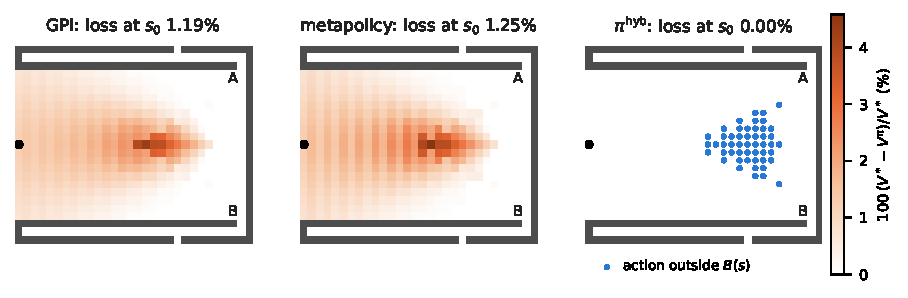
\includegraphics[width=\linewidth]{figures/hyb_example_windy.pdf}
\caption{Why the metapolicy: automaton state $u_0$ of the windy task ``($A$ or $B$), then a corridor exit'', where both
exits are worth the same, $\w(u_0)=(0.63,0.63,0,0,0,0)$. Colour: loss $V^*-V^\pi$ of each policy built from the 6
extremes, relative to $V^*$, at every state of the windy zone (start $\bullet$, exits $A$, $B$ on the right).
$\pi^{\mathrm{hyb}}$ takes the action RIGHT, which no extreme takes, at the blue states.}\label{fig:hedge}
\end{figure}

\paragraph{Why the metapolicy: hedging.} In the windy two-stage domain \cite{note} the wind decides whether the agent
reaches exit $A$ or $B$, and from each of them corridors lead to further exits. In a task such as ``($A$ or $B$), then a
corridor exit'' both exits are worth the same in $u_0$ (Figure~\ref{fig:hedge}). The optimal policy hedges: it moves
forward without pushing up or down, and commits only when the wind has decided. Each extreme pushes towards its own exit
from the first step. GPI evaluates every action followed by a \emph{single} extreme, so it never values waiting, and
loses $1.19\%$ at the start. The metapolicy switches between the extremes at every state (``up if the wind pushed us
up''), but each of them still pushes, so it loses $1.25\%$. $\pi^{\mathrm{hyb}}$ evaluates each action followed by the
\emph{metapolicy}: the one action outside $B(s)$ that matters, RIGHT (advance without choosing a side), is now valued
with a continuation that commits later, and $\pi^{\mathrm{hyb}}$ takes it at 50 central states. Its loss is 0 at the
start and at most $0.04\%$ anywhere. The metapolicy is therefore not useful as a policy but as the
\emph{continuation} that makes one non-base action enough, which a single base policy is not.

\paragraph{Certificate.} A policy is optimal for $\w$ iff its Bellman gap $\max_a[r_\w+\gamma PV^\pi](s,a)-V^\pi(s)$
is zero at every state. Checking it costs one evaluation of $\pi$ and one lookahead (prediction, no control), and
policy iteration detects it when it stops. Algorithm~\ref{alg:task} tries the cheap candidates first and only then
improves.

\begin{algorithm}[h]
\caption{SF-FSA-VI over a base $L$ in a stochastic domain}\label{alg:task}
\begin{algorithmic}[1]
\For{$u$ in reverse topological order}
  \State $\w(u)\gets$ exit weights: $1$, $V_v(i)$ (value of the policy executed in $v$) or $0$
  \State $\pi\gets$ GPI over $L$ at $\w(u)$;\ \ $V\gets$ evaluate $\pi$ \Comment{rung 1: zero-shot}
  \If{Bellman gap of $(\pi,V)$ is nonzero}
    \State $\pi\gets\pi^{\mathrm{hyb}}$ at $\w(u)$;\ \ $V\gets$ evaluate $\pi$ \Comment{rung 2: metapolicy, then $\pi^{\mathrm{hyb}}$}
    \While{Bellman gap of $(\pi,V)$ is nonzero} \Comment{rung 3: improve}
      \State $\pi\gets$ greedy for $r_\w+\gamma PV$;\ \ $V\gets$ evaluate $\pi$
    \EndWhile
  \EndIf
  \State execute $\pi$ in $u$;\ \ $V_u\gets V$
\EndFor
\end{algorithmic}
\end{algorithm}
\noindent By induction over the automaton, the executed policy is optimal and the planned values are exact.
Evaluations are iterative and warm-started at a sub-solution of the evaluated policy (the GPI estimate, $\max_jV_j$,
$V_{\mathrm{meta}}$), so no linear system is solved. \emph{Without the model}, rungs 2--3 become one Q-learner at
$\w(u)$, initialised at the GPI estimate, with acting and bootstrapping restricted to $B(s)$ (the metapolicy) and every
entry keeping the visit count of the base entry it was copied from (\emph{inherited counts}); otherwise the first noisy
updates overwrite an initialisation that is already near-optimal. The base itself is built once with
Certify-or-Grow \cite{cog}, or is just the $d$ extremes.

\section{Results}
Domains: double slit (wind $\pm3$, $\gamma=0.9$), Office with slip $p$ (the chosen action is replaced by one of the
other three w.p.\ $p$, $\gamma=0.99$) and windy two-stage ($\gamma=0.95$) \cite{note}. Office tasks: the 3 of
\cite{kuric}, \emph{sequential} ($C$, then $M$, then $O$), \emph{disjunction} ($C$ or $M$, then $O$) and
\emph{composite} ($C$ then $M$, or $M$ then $C$, then $O$), plus 100 random acyclic automata (up to 4 states, 1--2
symbols per state). Windy: 60 tasks ``($A$ or $B$), then 1--2 corridor exits'' (52; $u_0$ hedges) or ``$A$ (or $B$),
then corridor exits'' (8). The base is always the $d=6$ extremes.

\begin{table}[!t]\centering\small
\caption{Algorithm~\ref{alg:task} with the model, per task type (number of tasks in brackets), base = the 6 extremes.
Max regret over the tasks, relative to the optimal value, of zero-shot GPI \cite{kuric}, the metapolicy and
$\pi^{\mathrm{hyb}}$ executed without certification; share of automaton states where Algorithm~\ref{alg:task} stops at
rung 1/2/3; average cost per task of the certified optimum in full sweeps ($|S||A|$ one-step backups; an evaluation
sweep counts $1/|A|$): value iteration from scratch (best tolerance, then policy iteration to zero gap), GPI followed
directly by policy iteration (rung 2 skipped), and Algorithm~\ref{alg:task}. $|U|$: automaton states per task.
Every certified plan has regret 0.}\label{tab:task}
\setlength{\tabcolsep}{3.6pt}
\begin{tabular}{llccccccccc}
\toprule
&&& \multicolumn{3}{c}{max relative regret, uncertified} & rungs (\%) & \multicolumn{3}{c}{sweeps per task, certified}\\
\cmidrule(lr){4-6}\cmidrule(lr){8-10}
domain & task type & $|U|$ & GPI & metapolicy & $\pi^{\mathrm{hyb}}$ & 1/2/3 & VI & GPI + PI & Alg.~\ref{alg:task}\\
\midrule
Office & sequential (1) & 3.0 & $6.4\cdot10^{-9}$ & 0 & 0 & 33/67/0 & 109 & 62 & 84\\
$p=0.1$ & disjunction (1) & 2.0 & $9.3\cdot10^{-6}$ & $1.2\cdot10^{-7}$ & 0 & 0/50/50 & 66 & 50 & 77\\
& composite (1) & 4.0 & $1.8\cdot10^{-5}$ & $9.2\cdot10^{-6}$ & $2.5\cdot10^{-6}$ & 25/50/25 & 147 & 94 & 154\\
& random (100) & 1.7 & $1.8\cdot10^{-5}$ & $2.1\cdot10^{-5}$ & $1.7\cdot10^{-5}$ & 7/85/8 & 58 & 32 & 52\\
\midrule
Office & sequential (1) & 3.0 & $4.9\cdot10^{-6}$ & 0 & 0 & 0/100/0 & 234 & 140 & 230\\
$p=0.3$ & disjunction (1) & 2.0 & $9.9\cdot10^{-5}$ & $5.3\cdot10^{-5}$ & $3.5\cdot10^{-8}$ & 0/50/50 & 144 & 95 & 175\\
& composite (1) & 4.0 & $3.3\cdot10^{-4}$ & $8.4\cdot10^{-4}$ & 0 & 0/100/0 & 282 & 190 & 348\\
& random (100) & 1.7 & $1.3\cdot10^{-3}$ & $1.6\cdot10^{-4}$ & $1.2\cdot10^{-6}$ & 19/76/5 & 117 & 66 & 111\\
\midrule
Windy & $A$ or $B$, then corr.\ (52) & 3.0 & $1.2\cdot10^{-2}$ & $1.2\cdot10^{-2}$ & 0 & 90/2/8 & 102 & 12 & 19\\
& $A$ only, then corr.\ (8) & 2.0 & 0 & 0 & 0 & 100/0/0 & 42 & 2 & 2\\
\bottomrule
\end{tabular}
\end{table}

\begin{table}[!t]\centering\small
\caption{Without the model: Office with slip $0.05$, base = the 6 extremes learned by SF Q-learning (2.5M steps
each, visit counts kept). Millions of environment steps per task until the greedy policy of every automaton state is
within $10^{-3}$ of the optimum at its entry states (checked by an oracle; budget 2M per automaton state, a state that
does not get there counts 2M). All learners are scalar Q-learning at $\w(u)$ with step $1/(n+1)^{0.7}$; 20 tasks
(24 distinct automaton states), 2 seeds; $|U|$: automaton states per task.}\label{tab:mf}
\begin{tabular}{lcccccc}
\toprule
& & & \multicolumn{2}{c}{GPI start, all actions} & \multicolumn{2}{c}{GPI start, metapolicy ($B(s)$)}\\
\cmidrule(lr){4-5}\cmidrule(lr){6-7}
task type & $|U|$ & from scratch & fresh counts & inherited counts & fresh counts & inherited counts\\
\midrule
sequential & 3.0 & 2.47 & 2.42 & 1.63 & 2.41 & \textbf{0.59}\\
disjunction & 2.0 & 2.31 & 2.10 & 1.65 & 1.93 & \textbf{1.40}\\
composite & 4.0 & 4.10 & 3.43 & 1.89 & 3.64 & \textbf{1.56}\\
random (17) & 1.5 & 0.75 & 0.58 & \textbf{0.38} & 0.69 & 0.39\\
all 20 tasks & & 1.08 & 0.89 & 0.58 & 0.99 & \textbf{0.51}\\
\bottomrule
\end{tabular}
\end{table}

\begin{figure}[!t]\centering
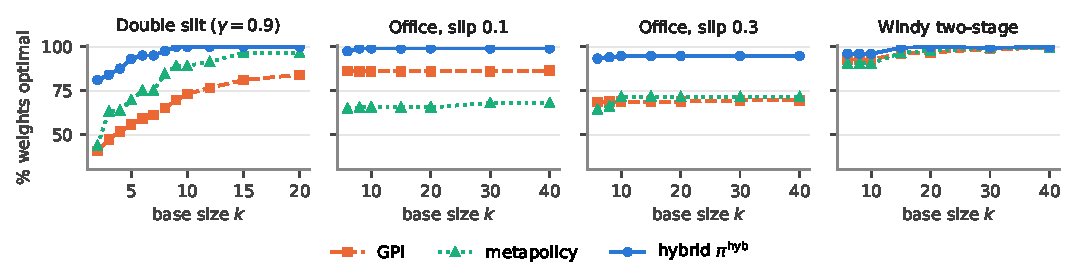
\includegraphics[width=\linewidth]{figures/hyb_optimal.pdf}
\caption{Share of held-out weights where each policy is optimal at the start and every exit, with the first $k$
policies found by OLS as base (the first $d$ are the extremes). Policy iteration from $\pi^{\mathrm{hyb}}$ reaches the
optimum in at most 3 steps (mean $\le0.3$) in every case.}\label{fig:opt}
\end{figure}

\begin{table}[!t]\centering\small
\caption{Building the $\epsilon$-CCS from the base (the $d$ extremes), with the model: average cost per CCS policy
beyond the base in SF sweeps ($|S||A|$ backups of $d$-dimensional SFs) and, in brackets, the policies trained beyond
the base.}\label{tab:ccs}
\begin{tabular}{lcccc}
\toprule
& Double slit, exact & Windy, $10^{-5}$ & Office 0.1, $2\cdot10^{-3}$ & Office 0.3, $5\cdot10^{-3}$\\
\midrule
CCS policies beyond the base & 308 & 111 & 256 & 232\\
SFOLS, learned from scratch & 889 (308) & 471 (111) & -- & --\\
SFOLS, GPI warm start & 20.7 (307) & 47.4 (111) & 57.2 (256) & 143.6 (232)\\
Certify-or-Grow & 21.3 (11) & 51.0 (15) & 60.0 (18) & 150.6 (16)\\
\bottomrule
\end{tabular}
\end{table}


\begin{itemize}\setlength\itemsep{2pt}
\item \textbf{Where the metapolicy matters (Table~\ref{tab:task}, Figures~\ref{fig:hedge} and~\ref{fig:opt}).} Where
GPI is already near-optimal there is nothing to fix: in Office with $p=0.1$ every policy is within $2\cdot10^{-5}$.
Where it is not, $\pi^{\mathrm{hyb}}$ fixes it: in Office with $p=0.3$, 9 of the 103 tasks lose more than $10^{-4}$
with GPI (up to $0.13\%$); the metapolicy brings 8 of them below $10^{-4}$ and $\pi^{\mathrm{hyb}}$ makes all 9 exact.
In windy, 12 of the 52 hedging tasks lose more than $10^{-4}$ (up to $1.2\%$); the metapolicy fixes none of them (it
cannot hedge, Figure~\ref{fig:hedge}) and $\pi^{\mathrm{hyb}}$ is exact on all 60. Over held-out weights (Figure~\ref{fig:opt}), GPI over the 6 extremes is
optimal at 86\%, 69\% and 93\% of them and $\pi^{\mathrm{hyb}}$ at 97\%, 93\% and 96\%; in double slit 9 policies
make $\pi^{\mathrm{hyb}}$ optimal everywhere, where the CCS has 181.
\item \textbf{Cost of the certified optimum, with the model (Table~\ref{tab:task}).} Every task is solved exactly.
The cheapest route is GPI followed directly by policy iteration: $1.8\times$ cheaper than value iteration from scratch
in Office and $8.6\times$ in windy (one evaluation certifies GPI in 90\% of the windy automaton states). With rung 2,
$\pi^{\mathrm{hyb}}$ is certified at 76--85\% of the Office automaton states, but its restricted policy iteration costs
more than the 2 improvement steps it saves, so Algorithm~\ref{alg:task} is $1.5$--$1.7\times$ more expensive than GPI
+ PI (about the cost of value iteration in Office). With the model, rung 2 buys a near-optimal policy before any
improvement step over all actions, not speed. GPI rarely passes the certificate in Office (8--18\%) although its
regret is tiny: the gap must vanish at \emph{every} state, also far from the task's entry states.
\item \textbf{Without the model (Table~\ref{tab:mf}).} Zero-shot GPI over the learned extremes is already within
$10^{-3}$ at 22 of the 24 automaton states, so the learner's job is mainly not to spoil it. With fresh counts it does:
two thirds of the runs that start optimal drift away, which costs $0.44$M steps per automaton state on average.
Inherited counts cut the cost per task $1.5$--$1.9\times$, and the metapolicy (restricting the learner to $B(s)$) helps most on the longer tasks:
$0.59$M instead of $1.63$M on the sequential task and $1.56$M instead of $1.89$M on the composite one, $0.51$M instead
of $0.58$M over all 20 tasks, $2.1\times$ fewer than learning from scratch (one learned base, 2 seeds: indicative).
\item \textbf{The CCS from the base (Table~\ref{tab:ccs}).} With the model, Certify-or-Grow trains 11--18 policies
instead of 111--308, at about the cost of warm-started SFOLS ($+3$--$8\%$ sweeps) and $9$--$42\times$ less than SFOLS
from scratch. Without the model (Figure~1 of \cite{cog} with SF Q-learning, Certify-or-Grow warm-starting its base
like SFOLS, 3 seeds) there is no reliable gain: in double slit (wind $\pm1$, $\epsilon=10^{-3}$) the metapolicies
converge in about 0 steps after the base, but the base is 80--100\% of the cost ($1.14\times$ fewer steps to converge
than warm SFOLS, $1.05\times$ model-free); in Office with slip $0.05$ ($\epsilon=0.05$), each metapolicy still needs about 1M steps,
Certify-or-Grow with the exact certificate falls back 14--23 times and needs $150$M steps against $129$M, and the
model-free certificate needs $112$M but accepts 14--18 metapolicies whose true gap exceeds the tolerance.
\item \textbf{Limits.} Rung 3 needs the model or a learner; certifying without the model is the open part (sampled
completion with 100 samples per pair wrongly certified 15--22\% of the metapolicies). The zero-gap certificate is
stricter than SF-FSA-VI needs; a certificate weighted by reachability from the entry states would let GPI stop at rung
1 far more often.
\end{itemize}

{\small
\begin{thebibliography}{9}\setlength\itemsep{0pt}
\bibitem{kuric} D.~Kuric, G.~Infante, V.~G\'omez, A.~Jonsson, H.~van~Hoof. Planning with a learned policy basis to
optimally solve complex tasks. ICAPS 2024.
\bibitem{cog} Certify-or-Grow, \texttt{paper/article.tex}.
\bibitem{note} Certified SF libraries, \texttt{notes/certified\_library.tex}.
\end{thebibliography}}
\end{document}
